\chapter{Identificarea bolilor cardiace cu re\c{t}ea neuronal\u{a}}

\^{I}nainte s\u{a} aplic\u{a}m o re\c{t}ea neuronal\u{a} peste setul nostru de date trebuie mai \^{i}nt\^{a}i s\u{a} le preproces\u{a}m pentru a le converti la un format mai adecvat, s\u{a} elimin\u{a}m unele date nedorite din setul de date care pot \^{i}ngreuna procesul de antrenare \c{s}i s\u{a} ad\u{a}ug\u{a}m unele date care ne vor fi folositoare pe parcurs.

\section{Preprocesarea datelor}

Deoarece datele furnizate de c\u{a}tre The National Heart, Lung, and Blood Institute sunt in format DICOM (Digital Imaging and Communications in Medicine), format destul de greu de lucrat, prima noastr\u{a} sarcin\u{a} va fi s\u{a} le convertim la un format mult mai propice, cum ar fi formatul PNG (Portable Network Graphics), pentru a putea cre\c{s}te viteza de calcul a re\c{t}elei neuronale. \^{I}nainte de a le convertii de la format DICOM la PNG putem s\u{a} mai extragem unele informa\c{t}ii de la fiecare radiografie pe care formatul DICOM le ofer\u{a}, cum ar fi spre exemplu  id-ul pacientului caruia \^{i}i apar\c{t}ine radiografia, numarul de linii \c{s}i de coloane a radiografiei, care definesc marimea , spa\c{t}iul \^{i}ntre pixeli, care reprezint\u{a} o pereche de numere care arat\u{a} distan\c{t}a fizic\u{a} dintre centrii a doi pixeli pe vertical\u{a}, respectiv orizontal\u{a}, acestea fiind m\u{a}surate in milimetrii, ad\^{a}ncimea radiografiei masurat\u{a} in milimetrii, pozi\c{t}ia imaginii, care reprezint\u{a} coordonatele pe axele x, y \c{s}i z, fa\c{t}\u{a} de col\c{t}ul de sus st\^{a}nga a imaginii a centrului  radiografiei facute, loca\c{t}ia relativ\u{a} a radiografiei reprezentat\u{a} in milimetrii \c{s}i axa de codificare a imaginii (dac\u{a} e pe coloan\u{a} sau pe r\^{a}nd ). Toate aceste informa\c{t}ii ne vor fi folositoare pe parcurs a\c{s}a c\u{a} le vom salva \^{i}ntr-un fi\c{s}ier CSV.

\par

Dup\u{a} citirea imaginii vom verifica dac\u{a} imaginea este orientat\u{a} pe coloan\u{a}, \^{i}n acest caz dac\u{a} este adev\u{a}rat  va trebuii s\u{a} calcul\u{a}m transpusa imaginii (liniile vor deveni coloane) \c{s}i s\u{a} o rotim pe orizontal\u{a} de-a lungul axei x, astfel \^{i}nc\^{a}t sus s\u{a} deivin\u{a} jos \c{s}i invers, jos s\u{a} devin\u{a} sus, astfel c\u{a} la final imaginea va fi rotit\u{a} cu 90 de grade iar dintr-o imagine orientat\u{a} pe coloan\u{a} vom avea o imagine orientat\u{a} pe r\^{a}nd. Imediat dup\u{a} aceea va trebuii s\u{a} redimension\u{a}m fiecare imagine astfel \^{i}nc\^{a}t fiecare s\u{a} aib\u{a} 256 de pixeli \^{i}n \^{i}n\u{a}l\c{t}ime \c{s}i 256 de pixeli \^{i}n l\u{a}\c{t}ime, acest lucru se va face prin decuparea uni patrat de 256 x 256 de pixeli din imaginea original\u{a} care s\u{a} cuprind\u{a} doar inima pacientului, pentru a realiza acest lucru prima dat\u{a} vom verifica dac\u{a} imaginea are dimensiunile mai mici dec\^{a}t dormi noi s\u{a} decup\u{a}m, dac\u{a} da atunci va trebuii s\u{a} adaug\u{a}m un border negru \^{i}n jurul imaginii astfel \^{i}nc\^{a}t s\u{a} atinge dimensiunea dorit\u{a}. Dup\u{a} ce ne-am asigurat c\u{a} imaginea are o \^{i}n\u{a}l\c{t}ime \c{s}i o l\u{a}\c{t}ime mai mare dec\^{a}t vrem noi s\u{a} decup\u{a}m  vom calcula punctele de start \c{s}i de final a decup\u{a}rii astfel \^{i}nc\^{a}t s\u{a} lu\u{a}m fix centrul imaginii, acesta este un compromis destul de bun av\^{a}n \^{i}n vedere faptul c\u{a} fiecare radiografie are inima pacientului situat\u{a} in mijlocul ei.

\par

Acum c\u{a} avem o imagine de dimensiune 256x256 va trebuii s\u{a} aplic\u{a}m metoda CLAHE (Contrast Limited Adaptive Histogram Equalization) pentru a \^{i}nbun\u{a}t\u{a}\c{t}i contrastul \c{s}i calitatea imaginii. CLAHE este o variant\u{a} \^{i}mbunat\u{a}\c{t}it\u{a} a tehnicii de egalizare a histogramei (Histogram Equalization) a unei imagini gri astfle \^{i}nc\^{a}t histograma aceasteia s\u{a} fie uniform\u{a} iar fiecare valoare care poate fi \^{i}ntr-o imagine gri s\u{a} aib\u{a} acela\c{s} num\u{a}r aproximativ de pixeli. Astfle c\u{a}, fie o imagine f cu $m_r$ linii \c{s}i $m_c$ coloane \c{s}i cu pixeli care au valor \^{i}ntre 0 \c{s}i 255, vom nota cu p ca fiind probabilitatea ca un pixel s\u{a} aib\u{a} valorea n.

$$p_n = \frac{\text{numarul de pixeli cu valoarea n}}{\text{numarul total de pixeli}}$$

Unde n are valori cuprinse intre 0 \c{s}i 255. Atunci metoda de egalizare a histogramei pentru un pixel dintr-o imagine gri la linia i \c{s}i la coloana c poate fi definit\u{a} \^{i}n felul urm\u{a}tor.

$$g_{i,j} = floor\bigg( 255 \sum_{n=0}^{f{i,j}} p_n \bigg)$$

\^{I}n formula de mai sus floor face rotunjirea la cel mai apropiat num\u{a}r \^{i}ntreg inferior, iar g reprezint\u{a} noua imagine derivat\u{a} din f care are histograma pixelilor egalizat\u{a}. Fa\c{t}\u{a} de tehnica de egalizare a histogramei care lucreaz\u{a} pe toat\u{a} imaginea, CLAHE aplic\u{a} acela\c{s} principiu doar c\u{a} pe un bloc de pixeli, spre exemplu un bloc de pixeli de dimensiune 8x8, dintr-o imagine, acest lucru este necesar pentru a evita schimbarea contrastului \^{i}n regiuni unde acest lucru ar duce la deteliorarea calita\c{t}ii imaginii.

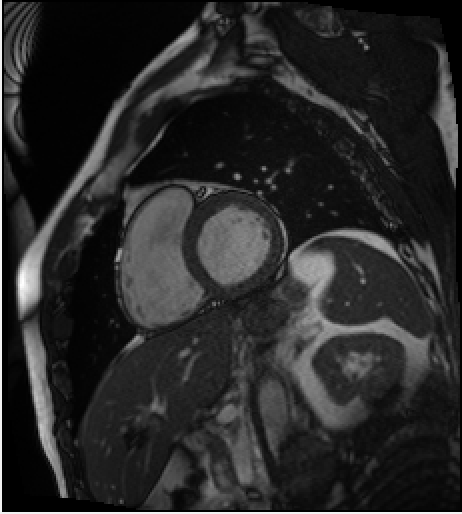
\includegraphics[width=150]{before.png}
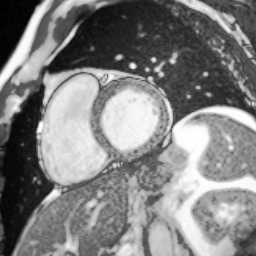
\includegraphics[width=150]{after.png}

Cele dou\u{a} imagini de mai sus reprezint\u{a} un exempu de imagine din setul de date \^{i}nainte de a fi procesat\u{a} \c{s}i dup\u{a} ce a fost procesat\u{a}, cum se poate observa imaginea procesat\u{a} a fost decupat\u{a} din mijlocul imaginii neprocesate astfel \^{i}nc\^{a}t s\u{a} se elimine o cantitate c\^{a}t mai mare de date care nu sunt necesare pentru scopul nostru, de asemenea se mai poate observa c\u{a} imaginea procesat\u{a} are un contrast mai mare fa\c{t}\u{a} de imaginea neprocesat\u{a} iar detaliile imaginii se pot observa mai bine, aceste lucruri vor duce la o vitez\u{a} de calcul \c{s}i la o acurate\c{t}e mai mare a re\c{t}elei neuronale.

\par

Cum am precizat mai sus, vom salva intr-un fi\c{s}ier CSV id-ul pacientului, numarul radiografiei, numarul imaginii, numarul de linii \c{s}i de coloane, distan\c{t}a fizic\u{a} \^{i}ntre centrii a doi pixeli, ad\^{a}ncimea radiografiei, locatia radiografiei, planul in care a fost facut\u{a} radiografia ( pe line sau pe coloan\u{a} ) \c{s}i pozi\c{t}ia imaginii fa\c{t}\u{a} de col\c{t}ul din st\^{a}nga sus, pe l\^{a}ng\u{a} toate acestea vom mai salva \c{s}i varianta prin care s-a facut radiografia, c\^{a}nd s-a f\u{a}cut radiografia, firma care a f\u{a}cut aparatul de RMN \c{s}i numele modelului, v\^{a}rsta pacientului, ziua de na\c{s}tere a pacientului, sexul pacientului, numele fi\c{s}ierului \c{s}i orientarea pacientului in imagine. DICOM define\c{s}te un sistem de coordonate numit RCS (Reference Coordinates System) prin care se stabile\c{s}te pozi\c{t}ia corpului  \^{i}n imagine, astfel c\u{a} direc\c{t}ia X este de la m\^{a}na dreapta a pacientului spre m\^{a}na st\^{a}ng\u{a} a acestuia, direc\c{t}ia Y este din fa\c{t}a pacientului spre spatele acestuia, iar direc\c{t}ia Z este de la picioare spre cap, din cauza faptului c\u{a} pozi\c{t}ia corpului este tridimensional\u{a} iar radiografia este bidimensional\u{a} se va caulcula proiec\c{t}ia fiecarei axe definite mai sus la axele unui plan bidimensional, \^{i}n acest caz \^{i}n formatul DICOM se vor gasi \c{s}ase valori care definesc orientarea pacientului in imagine. Primele trei valori reprezint proiec\c{t}ia celor trei axe a planului tridimensional la axa X a planului bidimensional (Xx, Xy, Xz), iar celelalte trei valori reprezint\u{a} proiec\c{t}ia celor trei axe a planului tridimensional la axa Y a planului bidimensional (Yx, Yy, Yz), cu aceste valori se poate stabilii foarte u\c{s}or cum este orientat un pacient intr-o radiografie.

\par

Toate valorile salvate mai sus \^{i}n fi\c{s}ierul CSV au fost valori pe care nu am fost nevoi\c{t}i s\u{a} le calcul\u{a}m doarece sunt deja existente \^{i}n fiecare radiografie, \^{i}ns\u{a} pe baza lor putem s\u{a} calcul\u{a}m noi valori care ne vor fi de folos pe parcurs. Una dintre acestea este s\u{a} stabilim timpul dintre dou\u{a} imagini consecutive dintr-o radiografie \c{s}i distan\c{t}a dintre loca\c{t}iile lor, acestea pot fi u\c{s}or calculate prin diferen\c{t}a dintre timpii  celor dou\u{a} imagini \c{s}i a pozi\c{t}iilor pe care le au.

\section{Identificarea inimii}

Cum se poate observa \c{s}i \^{i}n imaginea de mai jos inima este destul de u\c{s}or de identificat cu ochiul libert pentru un om, \^{i}ns\u{a} pentru un calculator aceasta este \^{i}nc\u{a} greu de g\u{a}sit.

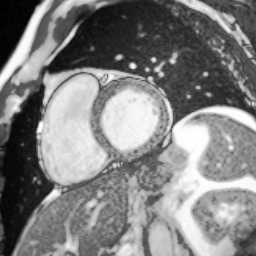
\includegraphics[width=200]{after.png}